\subsection{Composition, Inheritance, and Static Methods}
\textit{Show how to use a common piece of logic from two different classes, in three different ways: 1) by composition, 2) by inheritance, and 3) by static method calls, discuss the tradeoffs.}

\subsubsection{Inheritance}\label{s:inheritance}
The easiest way to think of class inheritance is that it is an "is-a" relationship. One class (child class) "is a" type of another class (super class).

For example, \texttt{Cat} and \texttt{Dog} classes are not the same, but they share common features. Both cats and dogs make a sound and they probably have a name. They have legs. We can abstract that common functionality into a super class called \texttt{Animal}.

\begin{figure}[H]\centering % Using \begin{figure*} makes the figure take up the entire width of the page
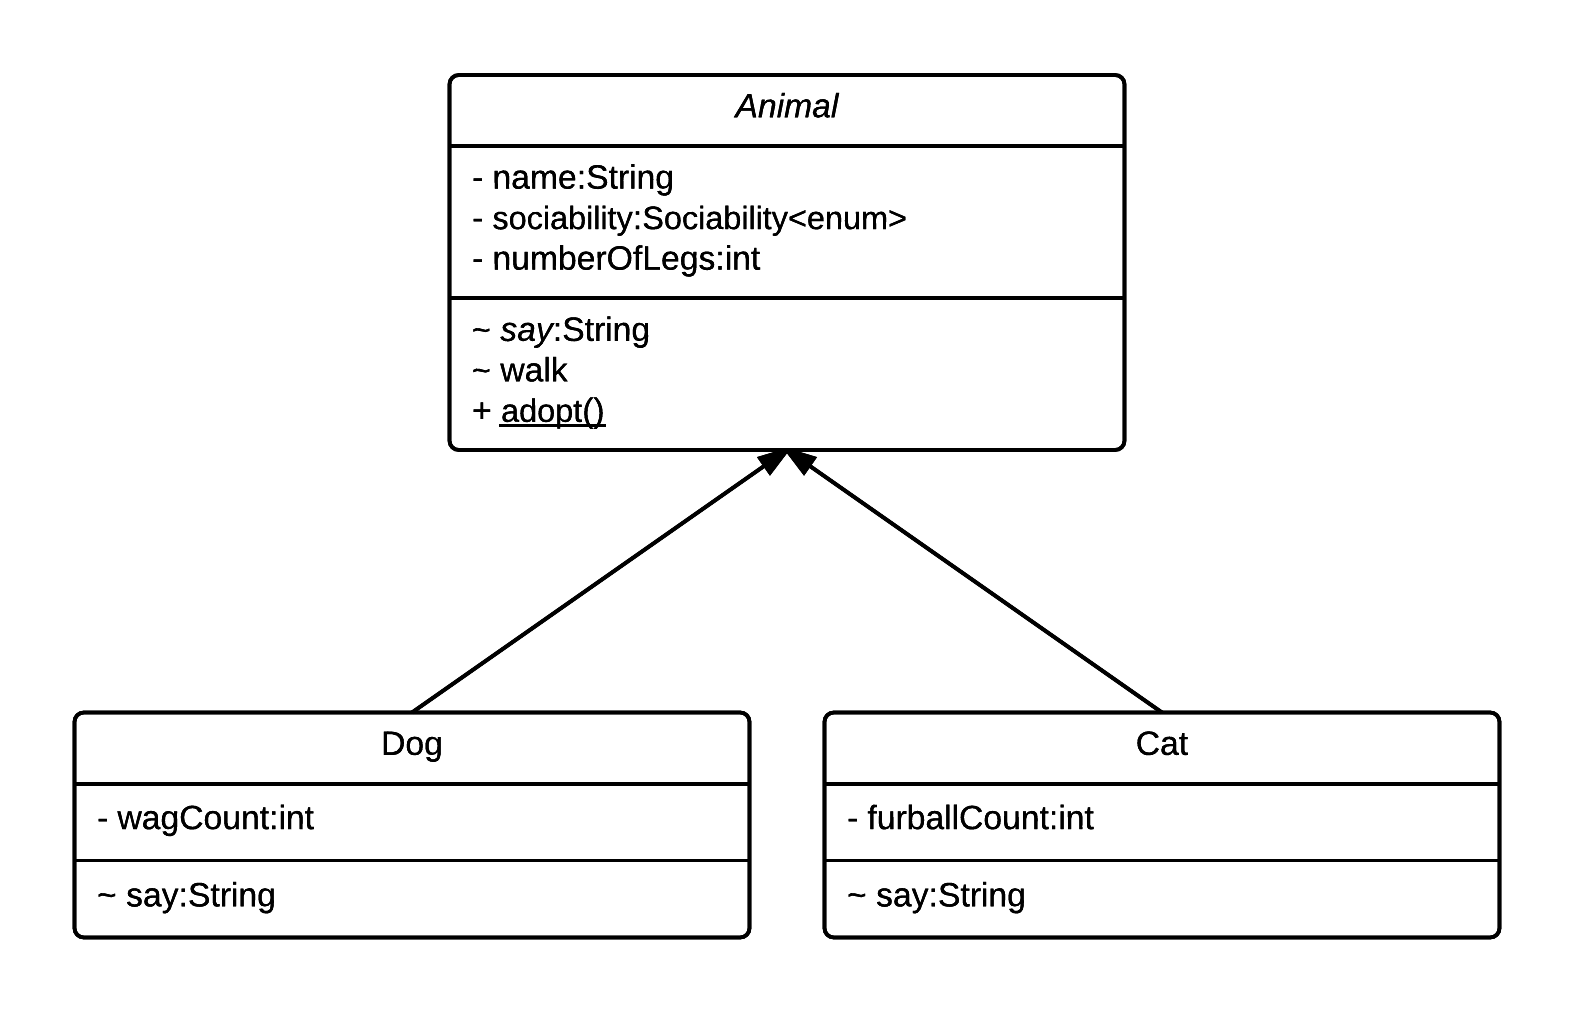
\includegraphics[width=0.9\linewidth, frame]{images/inheritance}
\caption{Inheritance ("Is-a")}
\label{fig:inheritance}
\end{figure}

We create the super class, \texttt{Animal} just like any other class:

\begin{lstlisting}[language=Java]
abstract public class Animal {
 private String name;
 private Sociability sociability;
 private int numberOfLegs;
 private Tail tail;

 public Animal(String name, int numberOfLegs, 
     Sociability sociability, Tail tail) {
  // initialize fields
 }

 // getters and setters...
 
 // toString...
}
\end{lstlisting}

We marked this class \texttt{abstract}. It will prevent any instantiation of the base class. The user of these classes has to instantiate a subclass of \texttt{Animal}. A super class does not have to be declared \texttt{abstract} unless it contains \texttt{abstract} methods (more about that later). We could allow the creation of super classes. In this case we opt not to.

Appendix J on page \pageref{App:AppendixJ} has the the source of the class \texttt{Animal.java}.

A \texttt{Dog} "is-an" \texttt{Animal}. The \texttt{Cat} "is-an" \texttt{Animal}. They inherit all protected and public methods and fields of \texttt{Animal}. See table \ref{tab:accessmodifiers} on page \pageref{tab:accessmodifiers} for details about access modifiers.

To create a child class, \texttt{Dog}, we simply create a class an extend from \texttt{Animal} using the \texttt{extend} keyword (line 1 in listing \ref{lst:dog}:

\begin{lstlisting}[language=Java, label=lst:dog]
public class Dog extends Animal {
 // ...
}
\end{lstlisting}

Cats and dogs also have unique features.  Cats have fur balls and dogs wag their tails. We can add fields and methods to the child class:
\begin{lstlisting}[language=Java]
// Dog: 
private int wagCount;

public int getWagCount() {
 return wagCount;
}

public void setWagCount(int wagCount) {
 this.wagCount = wagCount;
}

// Cat:
private int furballCount;

public int getFurballCount() {
 return furballCount;
}

public void setFurballCount(int furballCount) {
 this.furballCount = furballCount;
}
\end{lstlisting}
Appendix J on page \pageref{App:AppendixJ} has the the source of the classes \texttt{Cat.java} and \texttt{Dog.java}.
We can now create \texttt{Cat}s and \texttt{Dog}s:
\begin{lstlisting}[language=Java]

Animal pluto = new Dog("Pluto", Animal.Sociability.VERY_SOCIAL, 3);
Animal sheba = new Cat("Sheba", 2);

// We can also create a Dog object
Dog pepper = new Dog("Pepper", Animal.Sociability.VERY_SOCIAL, 99);

\end{lstlisting}

The difference between \texttt{pluto} and \texttt{pepper} is that the \texttt{pluto} reference is of type \texttt{Animal}, and the \texttt{pepper} reference is of type \texttt{Dog}. There usually isn't a good reason to use the specific reference (\texttt{pepper}). It conceptually goes against the purpose of inheritance.

If the super class has any public or protected methods, the child classes can call them. For example, if \texttt{Animal} has a method walk:
\begin{lstlisting}[language=Java]
protected String walk() {
 String steps = this.getName() + " walks: ";
 for (int i = 0; i < numberOfLegs; i++) {
  steps += " step";
 }
 return steps;
}
\end{lstlisting}

It simply writes "step" once for each leg.

We can call it from the \texttt{Dog} and \texttt{Cat} classes:

\begin{lstlisting}[language=Java]
// Inside a method in Cat:
String whatDoesTheCatSay = "Meouw ";
whatDoesTheCatSay += super.walk();
\end{lstlisting}

The \texttt{super} reference is optional (line 2). We could as well call the \texttt{walk()} method without it. After all a \texttt{Cat} "is-an" \texttt{Animal}. Using the \texttt{super} keyword makes the code clearer to read, though.

Executing the above code produces:
\begin{lstlisting}
Bark Pluto walks:  step step step step
Meouw Sheba walks:  step step step step
\end{lstlisting}


Since the child classes inherit the super classes public and protected members, we can call the \texttt{walk()} method from a reference:

\begin{lstlisting}[language=Java]
Animal spot = new Dog("Spot");

// Using a Dog reference works as well:
// Dog spot = new Dog("Spot"); 

spot.walk();
\end{lstlisting}

The output is:

\begin{lstlisting}
Spot walks:  step step step step
\end{lstlisting}

There is no way to force \texttt{Dog} call the \texttt{walk()} method. It is available for the child classes but they don't have to use it. If there is something that we want to enforce, there is a better way.

In \texttt{Animal} we can specify an abstract method \texttt{say()}. This way we force an \texttt{Animal} to have that functionality, but we force the child classes to specify what it means. 
\begin{lstlisting}[language=Java]
public abstract String say();
\end{lstlisting}

The method signature includes the \texttt{abstract} keyword, and there is no method body. The body will be implemented in each child class. In order to make a method \texttt{abstract} we also must mark the class \texttt{abstract} because there is no sense to instantiate an object that doesn't have a method implementation.

Although \texttt{Animal}s say things, they say different things. Dogs bark and cats meow. In the child classes we override the \texttt{say} method and implement it appropriately for each child class:
\begin{lstlisting}[language=Java]
// Dog:
@Override
public String say() {
 String whatDoesTheDogSay = "Bark";
 for (int i = 0; i < wagCount; i++) {
  whatDoesTheDogSay += " (wag) ";
 }
 whatDoesTheDogSay += super.walk();
 return whatDoesTheDogSay;
}
  
// Cat:
@Override
public String say() {
String whatDoesTheCatSay = "Meouw";
 for (int i = 0; i < furballCount; i++) {
  whatDoesTheCatSay += " (cough) ";
 }
 whatDoesTheCatSay += super.walk();
 return whatDoesTheCatSay;
}
\end{lstlisting}
Providing an alternate implementation of a method in the child class is called overriding. The overriding method has to have the same signature (return type and parameter list) as the method in the parent class. Java provides an annotation for marking a method overridden, namely \texttt{@Override}. If we use it and our method doesn't match the parent method, we will see an error. The annotation is useful for keeping us in check when overriding methods.

The \texttt{Dog} says "Bark", then wags the tail as many times as indicated by the wagCount, then walks (by calling the \texttt{super.walk()} method).

The \texttt{Cat} says "Meouw", coughs some furballs, and also walks.

We can create an \texttt{Animal} of type \texttt{Dog} and call the \texttt{say} method:

\begin{lstlisting}[language=Java]
Animal pepper = new Dog("Pepper", Animal.Sociability.VERY_SOCIAL, 99, new Tail(true, 1));
System.out.println(pepper.say());

Animal sheba = new Cat("Sheba", 2, new Tail(false, 15));
System.out.println(sheba.say());
\end{lstlisting}


When we call the \texttt{say} method we have the following output:
\begin{lstlisting}
Bark (wag)  (wag) ... (wag)
  Pepper walks:  step step step step

Meouw (cough)  (cough)
  Sheba walks:  step step step step
\end{lstlisting}

By forcing the child classes to implement a method, the super class can call it. Even when the \texttt{say()} method is not implemented in the \texttt{Animal} class, we can call it on an \texttt{Animal} reference. The JVM will find the appropriate implementation and execute that. This is called "virtual method invocation".

One of the benefits of inheritance is that we can treat Cat and Dog objects the same way, as instances of the Animal class. With that, we can, for example, store Cats and Dogs in the same collection and iterate through them.
\begin{lstlisting}[language=Java]
List<Animal> pets = new ArrayList<Animal>();
pets.add(spot);
pets.add(sheba);

System.out.println("\n\nAnimals in a list");
for(Animal animal : pets){
 System.out.println(animal);
}
\end{lstlisting}

The output looks like:
\begin{lstlisting}
Animal:{  
 name='Spot',
 sociability=VERY_SOCIAL,
 numberOfLegs=4,
 tail=Tail      {  
  docked=false,
  length=8
 }
}
Bark (wag)  (wag)  (wag)  (wag)  (wag) 
Spot walks:step step step step,

Animal:{  
 name='Sheba',
 sociability=VERY_UNSOCIAL,
 numberOfLegs=4,
 tail=Tail      {  
  docked=false,
  length=15
 }
}
Meouw (cough)  (cough)
Sheba walks:step step step step
\end{lstlisting}

See Appendix J on page \pageref{App:AppendixJ} for full source code of the \texttt{InheritanceCompositionExample.java} class.

Restricting access to a super class method or field is not allowed. Let's imagine we want to make a \texttt{Cat} that cannot be modified. We extend from \texttt{Cat}:
\begin{lstlisting}[language=Java]
public class ImmutableCat extends Cat {
// ...
}
\end{lstlisting}

If we try to override the setter for furballs, we get a compilation error:
\begin{lstlisting}[language=Java]
// does not compile
@Override
private void setFurballCount(int furballCount) {
 // don't let them set it
}
\end{lstlisting}

We cannot override with weaker access privileges than the super class. See Appendix J on page \pageref{App:AppendixJ} for full source code of the \texttt{ImmutableCat.java} class.

\subsubsection{Composition}
\begin{figure}[!h]\centering % Using \begin{figure*} makes the figure take up the entire width of the page
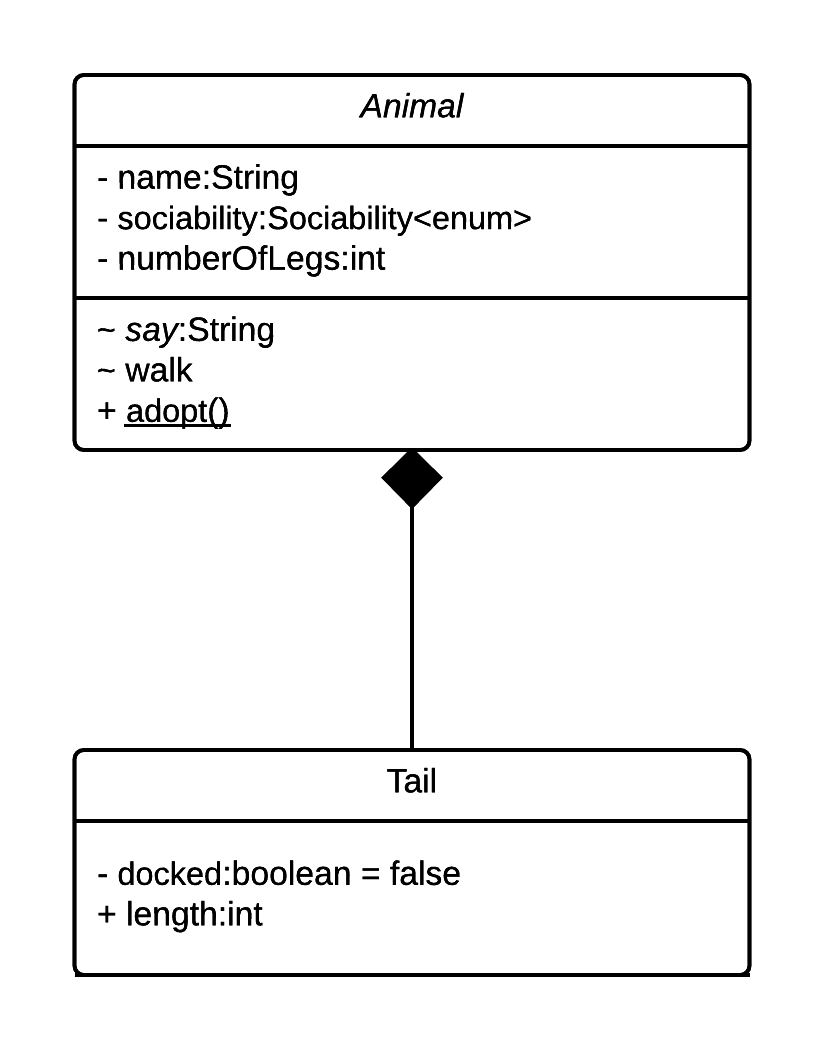
\includegraphics[width=0.9\linewidth, frame]{images/composition}
\caption{Composition ("Has-A")}
\label{fig:composition}
\end{figure}

A composition is another way to share features between classes. The easiest way to think of it is a "has-a" relationship. For example, a \texttt{Cat} and a \texttt{Dog} "have-a" \texttt{Tail}.

First we create a \texttt{Tail} class.
\begin{lstlisting}[language=Java]
public class Tail {
 private boolean 	;
 private int length;

 public Tail(boolean docked, int length) {
  this.docked = docked;
  this.length = length;
 }
}
\end{lstlisting}

We can make the \texttt{Animal} class "have-a" tail (although not all animals have tails, we simplify it for the sake of the example). Because \texttt{Dog} "is-an" \texttt{Animal}, it also "has-a" \texttt{Tail}. The same for the \texttt{Cat}.

Appendix J on page \pageref{App:AppendixJ} has the source code for the  \texttt{Tail.java} class.

We just create a field in the \texttt{Animal} class for the tail.
\begin{lstlisting}[language=Java]
private Tail tail;
\end{lstlisting}

Now we can access it from \texttt{Dog} or \texttt{Cat}, as well as from \texttt{Animal}:
\begin{lstlisting}[language=Java]
Tail tail = new Tail(false, 10);
pluto.setTail(tail);
System.out.println(pluto.getTail().isDocked());
\end{lstlisting}

The above code will output \texttt{false} because \texttt{pluto}'s tail is not docked.

\subsubsection{Static Methods}
There is yet another way to provide common functionality among several classes. We can declare a method or field \texttt{static}d:

\begin{lstlisting}[language=Java]
public static String adopt(){
 return "Yay! Adopted Animal!";
}
\end{lstlisting}

The \texttt{static} keyword makes the class, field, or method special. We don't need to instantiate an object to access \texttt{static} members of a class. They are class-level parameters and fields:
\begin{lstlisting}[language=Java]
System.out.println(Animal.adopt());

// displays
Yay! Adopted Animal!
\end{lstlisting}
We can access the \texttt{static} \texttt{adopt()} method from the class, without using the \texttt{new} keyword to create an object.

A class might want to provide \texttt{static} fields, for example constants. In such case they should be also marked \texttt{final}, to avoid modification.

Also anything that we might want to share between objects of the same class should be marked \texttt{static}. For example, we might (for some strange reason) want to keep a count of instances of a class. If we declare a \texttt{static} field, all instances of the class will access exactly the same copy of that field. If one modifies it, it will be also show modified for the other instances (unless it is marked \texttt{final}, in which case it can't be modified).

\subsubsection{Inner Classes}
It is worth mentioning one more way of sharing code between classes. In Java we can have inner classes, or classes inside of other classes. They have access to all the fields and methods of the outer class, including the private members.

An inner class can be instantiated from outside the outer class, if its access modifiers are set properly. But, the instantiation has to happen through an object of the outer object:
\begin{lstlisting}[language=Java]
OuterClass outer = new OuterClass();
OuterClass.InnerClass inner = outer.new InnerClass();
\end{lstlisting}

The inner object now has access to everything in the outer class. We could create two or more inner classes this way, and they all have access to common methods and fields in the outer class. 

It is not an "is-a", nor a "has-a" relationship. In some ways it breaks encapsulation and doesn't really look like object-oriented programming at all.